\documentclass[../p023main.tex]{subfiles}
\graphicspath{{\subfix{../figures/}}}

\begin{document}

\chapter{Einstein's Postulates}
\section{Einstein's Postulates}
All of special relativity is derived from two postulates.
\begin{enumerate}
    \item The laws of physics are the same in all inertial (i.e., constant-velocity) frames of reference.
    \item The speed of light $c$ is the same in all frames of reference.
\end{enumerate}
Both of these claims have mounds of experimental evidence to back them up.
They seem innocent enough at first glance, but together they lead to a rich and wildly intuitive theory of how the universe works.

\section{Time Dilation}
Suppose we're on a spaceship equipped with a light clock.
This light clock consists of two mirrors spaced a distance $D_0$ apart, with a beam of light bouncing back and forth between them.
\begin{center}
    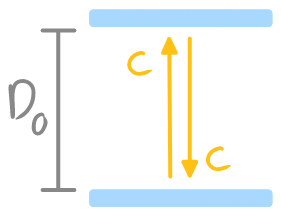
\includegraphics[width=0.25\textwidth]{statLightClock.png}
\end{center}
This clock ``ticks'' every time the light beam hits the bottom mirror.
From the equation $d = rt$, we can find the time $\Delta t_s$ between ticks:
\[ 2D_0 - c \Delta t_s \implies \Delta t_s = \frac{2D_0}{c}. \]
Now imagine another observer watches this spaceship (and the clock on it) fly past Earth at some speed $V$.
From the perspective of this observer, the light clock looks a little different.

The light, of course, is still bouncing between the mirrors; however, in order to ``keep up'' with the mirrors, the light now appears to travel \textit{diagonally} rather than straight up and down.
But remember, Einstein's postulates say that light must always travel at $c$, no matter the perspective.
No faster, no slower.
Just $c$.
\begin{center}
    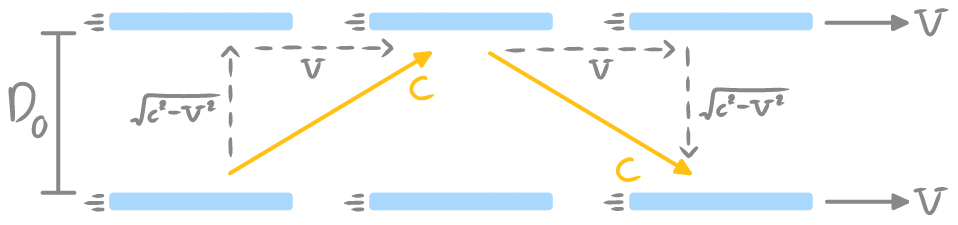
\includegraphics[width=0.9\textwidth]{transLightClock.png}
\end{center}
Is the time between ticks for the observer on Earth the same as it is for the observer on the spaceship?
To determine this, note that the beam of light bounces back and forth between the mirrors with vertical speed $\sqrt{c^2 - V^2}$.
Using the same $d = rt$ relationship, we can find the time $\Delta t_m$ between these new ticks:
\[ 2D_0 = \sqrt{c^2 - V^2} \cdot \Delta t_m \implies \Delta t_m = 2D_0 \cdot \frac{1}{\sqrt{c^2 - V^2}}. \]
We can see right away that this expression doesn't match the one for $\Delta t_s$, but how do the two compare?
To find out, let's do a bit of algebraic manipulation.
\begin{align*}
    \Delta t_m &= 2D_0 \cdot \frac{1}{\sqrt{c^2 - V^2}} \\
    &= \frac{2D_0}{c} \cdot \frac{1}{\sqrt{1 - \left( V / c \right)^2}} \\
    &= \Delta t_s \cdot \frac{1}{\sqrt{1 - \left( V / c \right)^2}}
\end{align*}
The expression $\sqrt{1 - \left( V / c \right)^2}$ is clearly less than one for $V < c$, making the above fraction greater than one.
Therefore, $\Delta t_m > \Delta t_s$.
Moving light clocks literally take longer to tick than stationary ones---even if they're otherwise identical!
Logical consistency requires that all accurate clocks, regardless of type, tick at the same speed, so we can make a generalization: moving clocks tick slowly by a factor of $\sqrt{1 - \left( V / c \right)^2}$.

This effect is called \textit{time dilation}---from the Earth's perspective, time itself runs slowly on the moving spaceship.
More precisely, if an undilated amount of time $t_0$ passes in our ``rest'' frame, then we perceive a moving object to have experienced the dilated time
\[ t = t_0 \sqrt{1 - \left( \frac{V}{c} \right)^2}. \]
Of course, the observer on the spaceship perceives themself to be the one at rest, so to them it is really our clock that is moving and thus running slowly.

\begin{summary}
    A clock that appears to move at a speed $V$ ticks slowly by a factor of $\sqrt{1 - \left( V / c \right)^2}$.
    That is, if it takes a time $t_0$ for a stationary clock to tick, the time it takes for a moving clock to tick is
    \[ t = t_0 \sqrt{1 - \left( \frac{V}{c} \right)^2}. \]
\end{summary}

\section{Length Contraction}
In our derivation of time dilation, we made an implicit assumption that the mirrors of our light click lay parallel to the direction of motion.
What if this were not the case?
More specifically, what would happen if your light clock instead moved downward rather than to the right?

Notice how (in the figure on the next page) I named the distance between the mirrors $D$ rather than $D_0$.
Given our unexpected conclusion about the passage of time, in the realm of relativity, we can no longer make any seemingly-obvious assumptions about the properties of moving objects.
More to the point, we will show that the distance $D$ between the moving mirrors is not $D_0$.

Let $\Delta t_d$ and $\Delta t_u$ be the amount of time the light spends moving downward and upward, respectively.
Using the figure above, we get the following $d = rt$ relationships.
\begin{align*}
    (D + v \Delta t_d) = c \Delta t_d &\implies \Delta t_d = \frac{D}{c - V} \\
    (D - v \Delta t_u) = c \Delta t_u &\implies \Delta t_u = \frac{D}{c + V}
\end{align*}
\begin{center}
    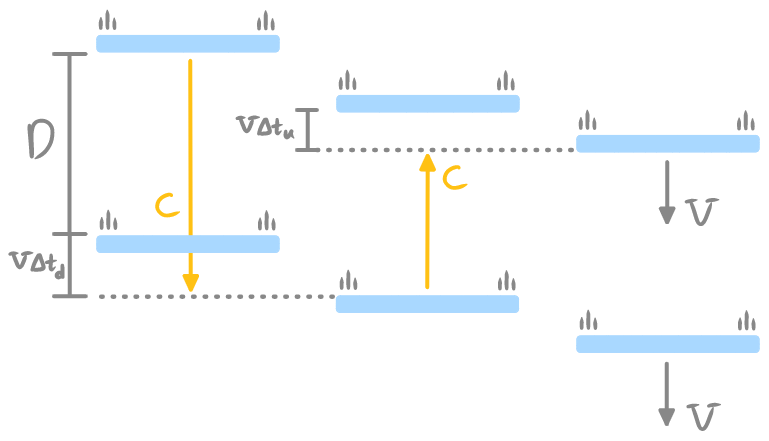
\includegraphics[width=0.8\textwidth]{longLightClock.png}
\end{center}
Since the total time $\Delta t_m = \Delta t_d + \Delta t_w$,
\begin{align*}
    \Delta t_m &= \Delta t_d + \Delta t_u \\
    &= \frac{D}{c - V} + \frac{D}{c + V} \\
    &= \frac{2Dc}{c^2 - V^2} \\
    &= \frac{2D}{c} \cdot \frac{1}{1 - \left( V / c \right)^2}
\end{align*}
Lastly, let $\Delta t_s = 2D_0 / c$ be the time it takes a stationary light clock to tick.
By time dilation,
\begin{align*}
    \Delta t_m &= \Delta t_s \cdot \frac{1}{\sqrt{1 - \left( V / c \right)^2}} \\
    \frac{2D}{c} \cdot \frac{1}{1 - \left( V / c \right)^2} &= \frac{2D_0}{c} \cdot \frac{1}{\sqrt{1 - \left( V / c \right)^2}} \\
    D &= D_0 \sqrt{1 - \left( \frac{V}{c} \right)^2}
\end{align*}
This effect is called \textit{length contraction}---from a stationary point of view, space itself becomes compressed for moving objects.
Note, however, that this only happens in the direction of motion, which is why length contraction was not a factor in our other setup.

\begin{summary}
    A length that appears to move at a speed $V$ is compressed by a factor of $\sqrt{1 - \left( V / c \right)^2}$ in the direction of motion.
    That is, if the length is $D_0$ when it is at rest, it becomes
    \[ D = D_0 \sqrt{1 - \left( \frac{V}{c} \right)^2} \]
    when it moves in a direction parallel to itself.
\end{summary}
\pagebreak

\section{Relative Simultaneity}
Let's imagine, again, that we're on a spaceship, this time equipped with two analog clocks spaced a distance $D_0$ apart.
In order to synchronize the clocks, a pulse of light is emitted from their midpoint so that it will reach each clock at the exact same time.
The clocks begin running when they detect the pulse.
\begin{center}
    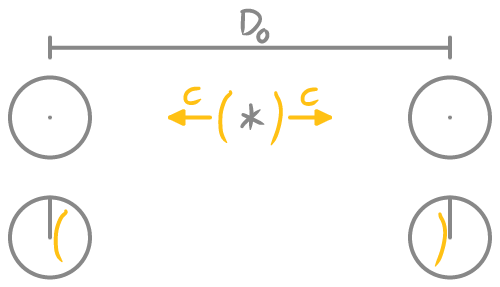
\includegraphics[width=0.5\textwidth]{restClockSync.png}
\end{center}
Clearly, from our perspective, the clocks will begin running simultaneously.
But what if we instead perceive the clocks to be moving, one following immediately after the other?
\begin{center}
    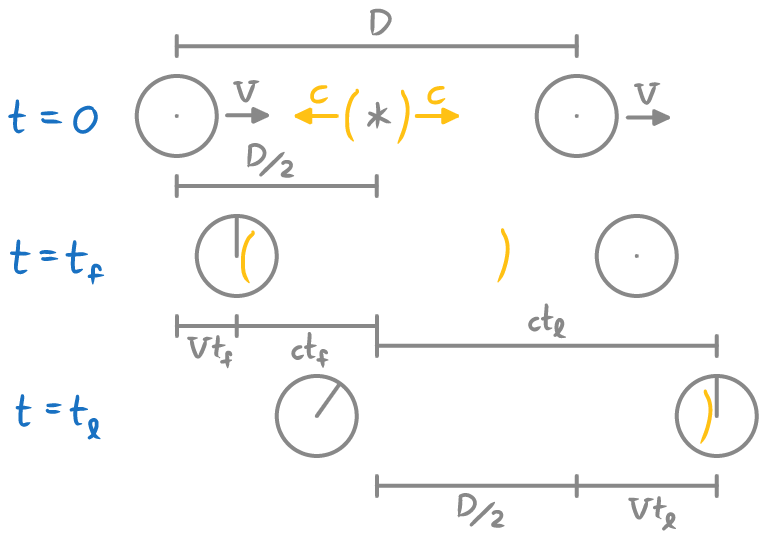
\includegraphics[width=0.8\textwidth]{movingClockSync.png}
\end{center}
One immediate change we see is the distance between the two clocks.
By length contraction, the distance between the moving clocks is $D = \sqrt{1 - \left( V / c \right)^2}$.
Not only that, but the beam of light will obviously reach the following (left) clock first, and \textit{then} the leading (right) one---these events, although simultaneous in one reference frame, are not simultaneous in another!
This is the relativity of simultaneity.
Now, let's quantify it.

Our aim, specifically, is to determine the difference $\Delta t$ between the times displayed by the clocks once they're both activated.
If the initial pulse is emitted at time $t = 0$, the light reaches the following clock at $t = t_f$ and the leading clock at $t = t_l$.
We can use the $d = rt$ relationships in the figure above to solve for these times.
\begin{align*}
    ct_f + Vt_f &= \frac{D}{2} & ct_l &= \frac{D}{2} + Vt_l \\
    (c + V)t_f &= \frac{D}{2} & (c - V)t_l &= \frac{D}{2} \\
    t_f &= \frac{D}{2(c + V)} & t_l &= \frac{D}{2(c - V)}
\end{align*}
From our perspective, the time difference between the two events is $\Delta t_0 = t_l - t_f$.
\begin{align*}
    \Delta t_0 &= t_l - t_f \\
    &= \frac{D}{2 (c - V)} - \frac{D}{2 (c + V)} \\
    &= \frac{DV}{c^2 - V^2} \\
    &= \frac{DV}{c^2 \left( 1 - \left( V / c \right)^2  \right)} \\
    \intertext{Since $D = D_0\sqrt{1 - \left( V / c \right)^2}$, this becomes}
    &= \frac{D_0 V \, \sqrt{ 1 - \left( V / c \right)^2 }}{c^2 \left( 1 - \left( V / c \right)^2  \right)} \\
    &= \frac{D_0 V}{c^2 \,\sqrt{ 1 - \left( V / c \right)^2 }}
\end{align*}
Finally, we must consider that the clocks are moving, and therefore tick slowly due to time dilation.
Therefore, the difference between the displayed times is
\begin{align}
    \Delta t &= \Delta t_0 \, \sqrt{ 1 - \left( \frac{V}{c} \right)^2} \\
    &= \frac{D_0 V \, \sqrt{ 1 - \left( V / c \right)^2}}{c^2 \, \sqrt{ 1 - \left( V / c \right)^2}} \\
    &= \frac{D_0 V}{c^2}
\end{align}
Note that this quantity is additive rather than multiplicative.
For example, if the following clock displays $t = \frac{D_0V}{c^2}$, then the leading clock will display $t = 0$.

\begin{summary}
    Events that occur simultaneously in one reference frame do not necessarily occur simultaneously in another frame.
    This is quantified by how, for two clocks moving at a speed $V$, the leading clock lags behind the other by an additive amount of $D_0V / c^2$, where $D_0$ is the rest length between the clocks.
\end{summary}

\section{The Lorentz Transformation}
So far we've used two simple postulates to derive three basic rules about the nature of spacetime: time dilation, length contraction, and relative simultaneity.
Here, we'll bring all of these rules together into one mathematical framework known as the Lorentz transformation in an effort to formalize everything we've talked about so far.
We'll then use it to see how to transform velocities between reference frames.

Let's begin with some terminology.
Consider two frames of reference called $S$ and $S'$.
By convention, we assume that the $S$ frame is at rest while the $S'$ frame moves in the positive $x$ direction with speed $V$.

Note that, in the figure on the next page, the $x$ and $x'$ axes should coincide---I just separated them slightly to distinguish the different frames.
For the remainder of this section, I will also omit the $z$ and $z'$ axes for clarity.
(Also, the primes on these coordinates have nothing to do with derivatives.
It's simply a way to denote the "transformed" version of each coordinate.)
\begin{center}
    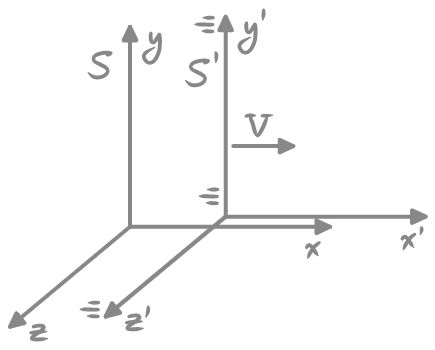
\includegraphics[width=0.4\textwidth]{movFrames.png}
\end{center}
Suppose an event $E$ occurs at a point in spacetime with $S$ coordinates $(t, x, y, z)$ and $S'$ coordinates $(t', x', y', z')$.
We'll use the three rules we've derived so far to determine the relationship between these sets of coordinates, starting with the spatial coordinates.
\begin{center}
    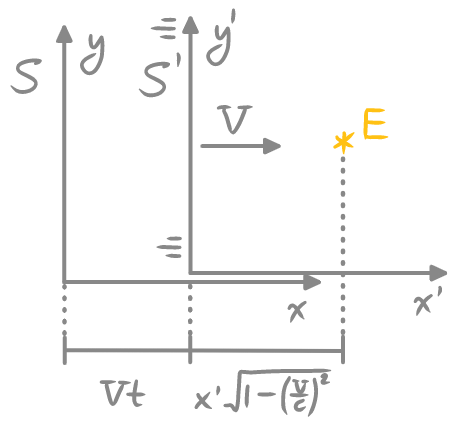
\includegraphics[width=0.4\textwidth]{movFramesSpat.png}
\end{center}
In the figure above, we are observing $E$ from within the $S$ frame.
We can decompose the $x$-coordinate of $E$ into two parts: the origin-to-origin distance between $S$ and $S$, and the distance from the $S'$ origin to $E$.

We know that the origin-to-origin distance is $Vt$, since the $S'$ frame has been traveling at a speed $V$ for a time $t$.
the distance between the $S'$ origin and $E$ appears to be $x'$, but recall that coordinates in the moving $S'$ frame are contracted, giving us $x' \sqrt{1 - \left( V / c \right)^2}$ for our distance.
Putting these two together, the $x$-coordinate of $E$ is
\[ x = Vt + x'\sqrt{1 - \left( \frac{V}{c} \right)^2}. \]
Solving for $x'$ gives the spatial transformation
\[ x' = \frac{x - Vt}{\sqrt{1 - \left( V / c \right)^2}}. \]
The $y$ and $z$ axes lay perpendicular to the direction of motion, so they aren't impacted by relativistic effects.
Their transformations are simply $y' = y$ and $z' = z$.

To transform between the temporal coordinates $t$ and $t'$, consider the same scenario from within the $S'$ frame.
The $S$ frame, along with the spatial location of $E$, is moving in the negative $x'$ direction at a speed $V$.
Also, the moment the two origins coincide, clocks stationed at each origin are synchronized with each other.
These are, in turn, used to synchronize all other clocks in their respective frames.

An observer at the origin of the $S'$ frame notices that a clock at the spatial position of $E$ ticks $Vx / c^2$ ahead of a clock at the origin of the $S$ frame.
(Remember---leading clocks lag.)
\begin{center}
    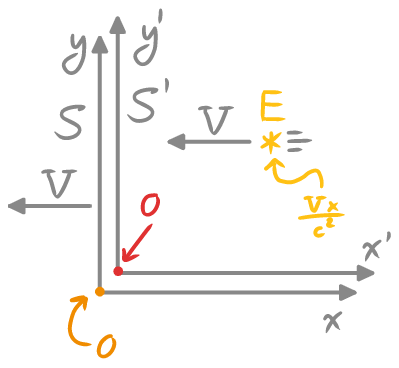
\includegraphics[width=0.4\textwidth]{movFramesTemp1.png}
\end{center}
As the $S$ frame continues to move, the event $E$ occurs at a time $t'$.
\begin{center}
    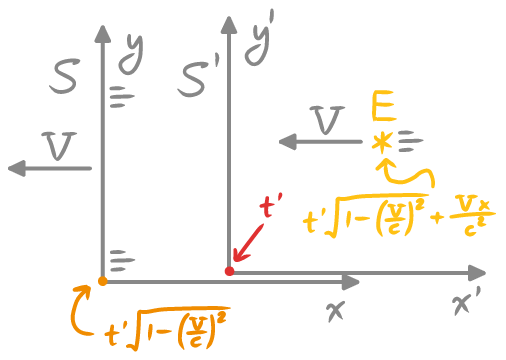
\includegraphics[width=0.5\textwidth]{movFramesTemp2.png}
\end{center}
Time in the moving $S$ frame is dilated, but we must be careful when we dilate---the phenomenon is only valid for clocks that have been previously synchronized, which in this case are the two clocks at the origins.
So, the clock at the origin of the $S$ frame reads $t' \sqrt{1 - \left( V / c \right)^2}$.
Finally, leading clocks lag, meaning a clock present for the event $E$ would read a time that is $Vx / c^2$ ahead of the origin clock.
So, in the $S$ frame, the event $E$ occurs at the time
\[ t = t' \sqrt{1 - \left( \frac{V}{c} \right)^2} + \frac{Vx}{c^2}. \]
Solving for $t'$ gives the temporal transformation
\[ t' = \frac{t - Vx / c^2}{\sqrt{1 - \left( V / c \right)^2}}. \]
Taken together, all these relationships comprise the Lorentz transformation.
This gives another, more formal way to analyze the behavior of spacetime, albeit less immediately intuitive.

The Lorentz transformation tells us how to transform positions in spacetime.
Transforming velocities is easy---we can just differentiate the Lorentz transformation equations!

Specifically, we'd like to relate the velocities $\left( \frac{dx}{dt}, \frac{dy}{dt}, \frac{dz}{dt} \right)$ and $\left( \frac{dx'}{dt'}, \frac{dy'}{dt'}, \frac{dz'}{dt'} \right)$ in the $S$ and $S'$ frames, respectively.
To do this, we simply take advantage of the chain rule for derivatives:
\begin{gather*}
    v_x' = \frac{dx'}{dt'} = \frac{dx'/dt}{dt'/dt} = \frac{v_x - V}{1 - Vv_x / c^2} \\
    v_y' = \frac{dy'}{dt'} = \frac{dy'/dt}{dt'/dt} = \frac{v_y\sqrt{1 - \left( V / c \right)^2}}{1 - Vv_x / c^2} \qquad
    v_z' = \frac{dz'}{dt'} = \frac{dz'/dt}{dt'/dt} = \frac{v_z\sqrt{1 - \left( V / c \right)^2}}{1 - Vv_x / c^2}
\end{gather*}
Take great care when using this velocity transformation!
It is assumed that the $S'$ frame moves to the right with respect to the $S$ frame.

\begin{summary}
    Let there be two reference frames $S$ and $S'$.
    The $S'$ frame moves with speed $V$ in the positive $x$ direction of the $S$ frame, and the frames' origins coincide at $t = t' = 0$.
    If an event occurs with $S$ coordinates $(t, x, y, z)$, then in the $S'$ frame these coordinates are given by the Lorentz transformation:
    \begin{align*}
        t' &= \gamma \left( t - \frac{Vx}{c^2} \right) \\
        x' &= \gamma \left( x - Vt \right) \\
        y' &= y \\
        z' &= z
    \end{align*}
    where $\gamma = \frac{1}{\sqrt{1 - \left( V / c \right)^2}}$ is the Lorentz factor.
    Differentiating these equations gives the velocity transformation:
    \begin{gather*}
        v_x' = \frac{dx'}{dt'} = \frac{dx'/dt}{dt'/dt} = \frac{(v_x - V)}{1 - Vv_x / c^2} \\
        v_y' = \frac{dy'}{dt'} = \frac{dy'/dt}{dt'/dt} = \frac{v_y}{\gamma \left( 1 - Vv_x / c^2 \right)} \qquad
        v_z' = \frac{dz'}{dt'} = \frac{dz'/dt}{dt'/dt} = \frac{v_z}{\gamma \left( 1 - Vv_x / c^2 \right)}
    \end{gather*}
\end{summary}
    
\end{document}